\section{Dataset}
The data we used was obtained from a deployment of sensors in a 12-story office building
on the campus of the University of Tokyo~\cite{gutp, ogawa:lncs2011}.  The deployment consists of 
1215 sensor monitoring device power consumption, ranging from plug-load devices to components of the
heating, ventilation, and air conditioning system and lighting.  Sensors also reported temperature
data, pressure, device-state, and other device information.  Each sensor reports data on the
order of minutes.  However, with the number of sensors, the collected data over a ~2 year
span was about half a terabyte.

% The intent of the Green University of Tokyo Project (GUTP) \cite{gutp} is to reduce the university environmental impacts associated to its electric energy consumption.
% The first step of this project was to deploy sensors at the Building No.2 of the Faculty of Engineering 
% Electric power consumption of a 12 floors building containing researchers office and classroom.
% 1215 sensors monitoring different devices...

%received attention in the past \cite{ogawa:lncs2011}.

For our investigation we focues on a three-week span in the summer of 2011 (from July 4th to July 24th).
The dataset capture regular work days, weekends and one holiday (July 18th).  This gave us a representative sample
of how the equipment is used for various activities as they are influenced by occupant schedules.  For the initial
analysis we also narrowed the search down to three sensors:

% includes one day holiday (July 18th)
% 3 different sensors:
\begin{itemize}
 \item 2 are measuring the electric power consumption of two devices from the same room; an Electric Heat Pump and the room lighting system.
 \item 1 is measuring the electric power consumption of a Gas Heat Pump that is heating and cooling a different room in the same building.
\end{itemize}

Later we expand our analysis to include all the sensors in the building.

\section{Problem statement}\label{problem}
Find device correlation at large spatial and time scales.

Usual measures on sensor data like correlation coefficient or granger causality \cite{kim:buildsys2010}
-- this is not working


\begin{figure}
 \subfigure[EHP]{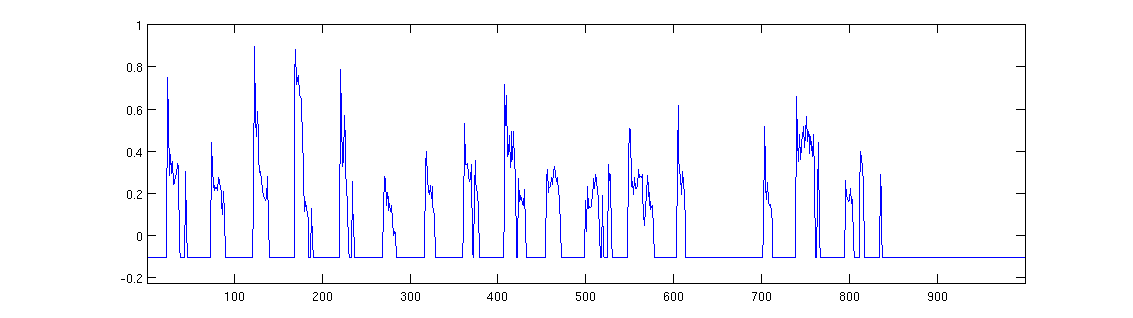
\includegraphics[width=.5\textwidth]{img/25.png}}
 \subfigure[Light]{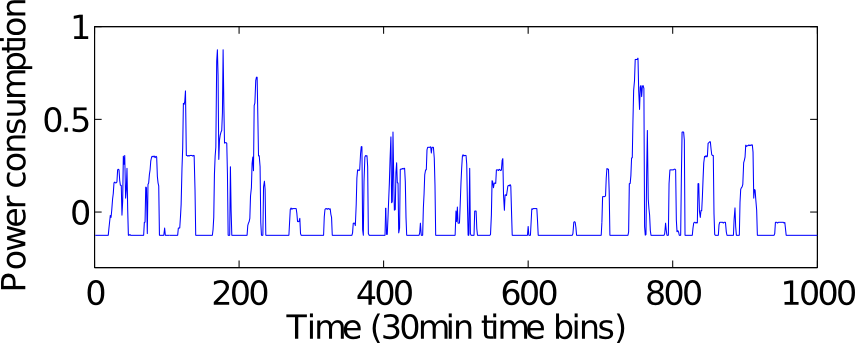
\includegraphics[width=.5\textwidth]{img/26.png}}
 \subfigure[GHP]{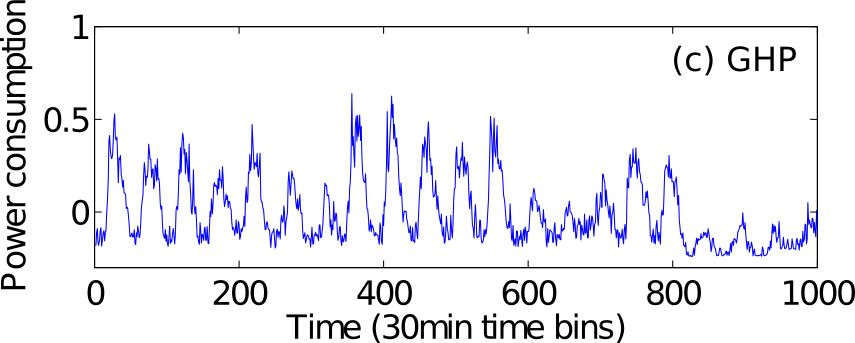
\includegraphics[width=.5\textwidth]{img/41.png}}
 \caption{Data from three different sensors captured in 2011 from July 4th to July 24th.}
 \label{fig:raw}
\end{figure}

For example correlation coefficients for the 3 signals...
correlation coefficient for the EHP and Light signals: $0.772013$
correlation coefficient for the EHP and GHP signals: $0.636967$

These scores suggest that the EHP signal is related to the two other measured signals.

These results were expected for the EHP and Light signals as the two measured devices operate for the same room and are used simultaneously.
These results, however, suggest that the EHP and GHP signals are highly correlated whereas in facts the two corresponding devices are located at two opposite sides of the building and their functioning is independent.
The small difference between the two computed correlation coefficients is misleading as one could conclude that the three signals are correlated and the corresponding devices are activated by a single action.

The high correlation coefficients obtained for these three signals result .... weekly pattern....
small difference = local fluctuation...

this high score comes from the fact that the two devices are monitoring offices that are weekly used.

Indeed the weekly pattern of the data trump the correlation coefficients....

How to inspect only the local fluctuations...?
we'd like to have an elegant solution (i.e. not specifying the interesting time scale)

